\documentclass[11pt]{article}

% use the free version of the Arial font
% \usepackage[scaled]{uarial}
% \renewcommand*\familydefault{\sfdefault} 
% \usepackage[T1]{fontenc}
% so installing arial gives problems for wsl running texlive
% switching over to just using helvetica to get around that issue
\renewcommand{\rmdefault}{phv} % Arial
\renewcommand{\sfdefault}{phv} % Arial

% pandas tables
\usepackage{booktabs}

% figure wrapping
\usepackage{wrapfig}
\usepackage{graphicx}
\graphicspath{ {./images/} }

% text box
\usepackage{amstext}

% set margins to be 0.5 in
\usepackage[legalpaper, portrait, margin=0.5in]{geometry}

% set all font sizes in this document to be size 11pt
\renewcommand{\tiny}{\normalsize}
\renewcommand{\footnotesize}{\normalsize}
\renewcommand{\small}{\normalsize}
\renewcommand{\large}{\normalsize}
\renewcommand{\Large}{\normalsize}
\renewcommand{\LARGE}{\normalsize}
\renewcommand{\huge}{\normalsize}
\renewcommand{\Huge}{\normalsize}


% reduce vertical space between headings
\usepackage[compact]{titlesec}
\titlespacing*{\section}{0pt}{*2}{*0}
\titlespacing*{\subsection}{0pt}{*1}{*1}
\titlespacing*{\subsubsection}{0pt}{*1}{*1}

% indent 1st paragraph
\usepackage{indentfirst}

% make references clickable
\usepackage{hyperref}

\begin{document}

\noindent
\textbf{Preliminary Exam Proposal} \hfill \textbf{Name:} Chinmay Raut \textbf{Dissertation Advisor:} Elizabeth Speliotes

\noindent
\textbf{Committee: } Margit Burmeister, Ryan Mills, Stephen CJ Parker, Maureen Sartor

\section*{\centerline{Studying the Effects of Rare Variants in Metabolic Syndrome}}

\section*{Specific Aims}

Metabolic syndrome (MetS) is a combination of 5 health risk factors, including abdominal obesity, high blood pressure, high triglycerides, low high-density lipoprotein (HDL) cholesterol, and high fasting blood sugar, that together increase the risk for cardiovascular disease, type 2 diabetes, stroke, and other chronic conditions \cite{pmid29480368}. MetS diagnosis is based on thresholds for these 5 quantitative traits, and individuals must surpass the thresholds on 3/5 of these traits for diagnosis making this a complex disease to study. Up to 1 in 3 Americans currently satisfy the MetS conditions making it a significant public health challenge \cite{pmid29480368}. The underlying mechanisms of metabolic syndrome are not fully understood but are thought to involve a genetic component with MetS having an estimated heritability of about 20-30\% \cite{Graziano2019}. There is a need for further research to determine the underlying causes of MetS and to develop effective strategies for prevention and treatment.

Previous studies have identified hundreds of associations between common genetic variants and MetS using Genome-Wide Association Studies (GWAS) on databases of up to 300,000 individuals \cite{pmid31589552}. However, little is known about the effects of rare variants on MetS, and no large-scale ($>$100,000 individuals) rare-variant associations have been conducted on MetS \cite{Lee2018}. Rare genetic variants (minor allele frequency $<$0.05) are worth studying for three reasons: they make up most of the sites of variation across the genome \cite{pmid34662886}, they are predicted to result in significant phenotypic changes if they reside in protein-coding regions \cite{pmid34662886}, and studying effects in protein-coding regions also provides a direct route for future functional studies and therapeutic targets \cite{doi:10.1056/NEJMoa2117872}. With the integration of Next-Generation Sequencing and longer read technology, genetic repositories like the UK Biobank (UKBB) recently released their Whole Exome Sequencing  (WES) data (26 million variants across 450,000+ individuals) resulting in high-quality data on low-frequency genetic variants \cite{pmid34662886}. Currently, studies on rare variants in GWAS are limited by power due to low sample counts of individuals within a selected rare variant. A series of approaches have been developed to combat these limitations including the construction of the optimal Sequence Kernel Association Test (SKAT-O) \cite{pmid22863193} which combines a set of rare variants together to increase the power of the association test. When the SKAT-O is paired with a variant annotator like the WGS Annotator (WGSA) \cite{pmid26395054} this results in the direct implication of genes to an outcome.

To understand the role genetic variants have on MetS, we want to identify and study its associations with rare, protein-coding variations using data from Biobanks. Exonic variants have the potential to alter proteins which then directly affect MetS phenotypes. Therefore, studying protein-altering variants offers direct insight into the biological mechanisms of MetS. We hypothesize that using WGS and WES data from large Biobanks such as the UKBB, we can detect exonic variants resulting in protein-coding changes which affect MetS. This will establish a series of protein-altering variants that provide insight into factors of MetS either for improvements in genetic testing or follow-ups for functional studies to investigate the biological mechanisms underlying the associations.

\subsection*{Aim 1: Determine Novel Gene-Based Associations with MetS.}

\textbf{Aim 1a: Identify genes associated with components of disease.} Since MetS diagnosis depends on 5 different quantitative traits(waist circumference, diastolic \& systolic blood pressure, triglycerides, HDL, and fasting blood glucose), we can extract each of those phenotypes from our discovery study cohort. We then run gene-based analysis techniques such as the SKAT-O to identify associations between genes and each of these MetS components.

\textbf{Aim 1b: Integrate discovered signals across components to study the holistic effect on disease.} After identifying significant genes across the 5 factors of MetS, we will conduct enrichment analysis on the gene-based results from Aim 1a genes associated with multiple MetS profiles. We will also perform gene-based association tests against a joint MetS diagnosis and severity score variables.

Based on the rare exonic variants we expect to identify and implicate specific genes that associate with components of MetS. We expect to construct a network of how these genes affect MetS as a whole, and if certain genes share similarities in effect on MetS providing further insights into its genetic basis.

\subsection*{Aim 2: Determine sequence-specific mechanisms of disease and progression.}

\textbf{Aim 2a: Within a gene, identify loci of individual variants affecting MetS.} We will perform Leave One Variant Out (LOVO) studies on the effects of variants within an implicated gene to understand if the effects of the protein-altering variants are restricted to a specific region of the gene or not.

\textbf{Aim 2b: Design CRISPR CAS9 KO guides based on exonic variants.} Based on the specific type of rare variants identified (frameshift, splicing, missense, etc…) we will design a CAS9 guide library surrounding those regions to study the functional effects of the identified variants in vitro.

We expect to produce a series of specific genomic loci potentially responsible for changes in MetS along with a CAS9 library for future functional experiments. This provides a direct target for future studies regarding the effects of genetic modification on MetS.

\

By studying new next-generation sequencing data to understand the role of rare genetic variants on MetS, we expect to identify genes that affect MetS and also provide biological insight into how they relate to the components of the condition. This study would lay the groundwork for further functional tests to investigate the biology behind the genetics of MetS and provide a genetics-based informatory tool to understand how one's genome contributes to risks in MetS.

\newpage

\subsection*{Background and Motivation}

Metabolic syndrome (MetS) is a combination of 5 health risk factors, including abdominal obesity, high blood pressure, high triglycerides, low high-density lipoprotein (HDL) cholesterol, and high fasting blood sugar, that together increase the risk for cardiovascular disease, type 2 diabetes, stroke, and other chronic conditions. ~33\% of Americans currently satisfy the MetS conditions making it a significant public health challenge. The underlying causes or biological processes behind MetS are not fully understood but the disease is thought to have a genetic component with a heritability estimate of 20-30\%. 

Genome-wide association studies (GWAS) are a powerful approach used in genetics research to identify genetic variations associated with complex diseases or traits. In a GWAS, researchers analyze the genetic information of large groups of individuals to identify genetic markers, or locations along the genome, that are associated with the disease or trait of interest. By comparing the frequency of these genetic markers between individuals with the disease or trait and those without, researchers can identify specific genetic variations that may relate to the development of the disease or trait. GWAS for MetS have identified a couple of promising candidate genes such as APOB, LPL, CETP, APOA5, GCKR, and ZNF259 to be associated with MetS incidence in large European populations ($>$300k individuals). These genes implicate lipid metabolism to be a major contributor of MetS. However, since 2 of the defining characteristics for MetS are defined by lipids (HDL and triglycerides) and these genes have a lesser impact on the other 3 characteristics of the disease, it suggests that these genes alone do not explain the entire genetic effect on MetS.

\begin{wrapfigure}{r}{0.6\textwidth}
  \begin{center}
    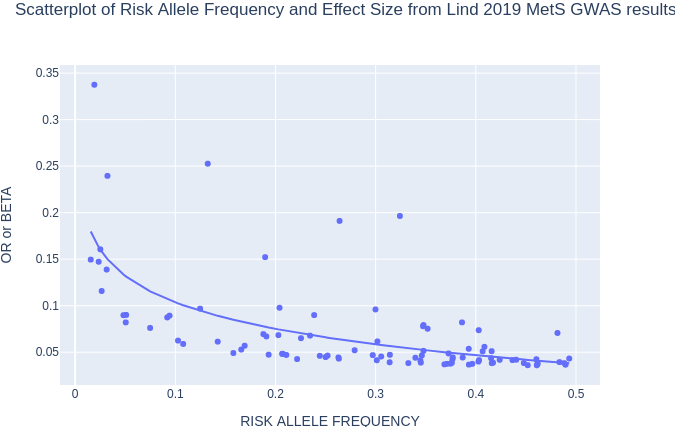
\includegraphics[width=0.60\textwidth]{"images/fig1v2.png"}
  \end{center}
  \caption{\textbf{Scatterplot of Risk Allele Frquency and Effect Size} (reconstructed from Lind 2019 MetS GWAS results). Effect size of variant increases inversely to allele frequency.}
  \label{fig:f1}
\end{wrapfigure}

Another limitation of most GWAS on MetS is that they are unable to detect associations between rare variants, defined as having a frequency of less than 1\% in the population. Previous studies tended to focus on common variants as this data is easier to acquire and study due to their increased imputation accuracy and prevalence in a population. However, one trend that has been identified through multiple GWAS is that rarer variants tend to have much larger phenotypic effects on an individual \ref{fig:f1}. There is potential that some of the large individual effects of genetic variants on MetS can be discovered through rare variant analyses. The primary problem of detecting rare variant associations lies within the rare nature of the variants. By definition, individuals with a selected rare variant make up less than 1\% of the population leading to massive sample size imbalances across carriers of a mutation vs non-carriers during the statistical tests. An alternative approach is to pool the effects of multiple rare variants, that we expect to behave similarly, together to combat the poor sample size imbalance. If we combine people that have any of multiple rare variants in an area we might have less imbalance of carrier vs non-carrier. One approach to this technique is known as the Optimal Sequence Kernal Association Test (SKAT-O). Most rare-variant associations use the SKAT-O in conjunction with variant annotation tools to test groups of variants belonging to the same gene or genomic region to directly implicate new genes with outcomes instead of specific point mutations. 

Advancements in sequencing technology have resulted in a technique known as Whole exome sequencing (WES) which is used to sequence the protein-coding regions of an individual's genome, also known as the exome. WES offers additional insight particularly for rare variant GWAS as it is known to be more accurate than genotyping or imputation due to its ability to reconstruct exact sequences from an individual. There have been a couple of studies looking at the rare-variant associations in MetS using WES data. A study focusing on about 10,000 individuals with Korean ancestry identified MetS associations with rare variants in the CETP region. However, this study faced some limitations particularly due to the smaller sample size compared to previous studies. Due to the relatively small effects of genetic variants, it is recommended to run GWAS on large populations to increase the power of the tests and their ability to detect suspicious loci.

Large biobanks such as the UK Biobank (UKBB) have recently released their WES data for a sample of over 450k European individuals. This offers the opportunity to study the effects of rare variants across a large cohort of individuals and perhaps discover novel protein-coding variants associated with MetS. One of the benefits of the UKBB WES data is that mutations observed are exonic which means that their implication with genes and proteins will be easier to study and assess compared to variants identified between 2 genes or in a non-coding region of the genome. We hypothesize that by studying rare variant associations through SKAT-O in MetS using the UKBB WES data, we can discover new genes or loci implicated with disease and further increase our understanding of the genetic factors associated with MetS.

\subsection*{Significance}

No large-scale (\>100k individuals) studies have been conducted on rare variants for MetS. Rare variants are important to study due to their relatively large phenotypic effects compared to common variants. An exome-wide analysis of rare variants associating with MetS can help identify protein-coding changes that are related to disease providing further biological insight into the mechanisms at play. Furthermore, such a study will allow for directed functional follow-up and potentially guide new therapeutic approaches to MetS.

\subsection*{Datasets}

\textbf{UK Biobank (discovery):} The UKBB large-scale population-based study consists of extensive health and lifestyle information from over 500,000 participants including various blood biochemistry data and sequence data. WES was performed on 454,787 participants across >26 million variants.

\textbf{Michigan Genomics Initiative (validation):} The MGI is a precision health research program based at the University of Michigan in Ann Arbor consisting of an opt-in study for hospital patients at the Michigan Medicine Hospital. This dataset consists of medical records for over 100,000 patients. Recently 70,439 individuals have been genotyped and imputed to the Trans-Omics for Precision Medicine (TopMed) rare variant reference panel consisting of \>50 million variants.


\subsection*{Research Design and Methods}

\subsection*{Aim 1: Determine Novel Gene-Based Associations with MetS.}

\subsection*{Aim 1a: Identify genes associated with components of disease.} 

\noindent \underbar{Rationale:}

Due to the complex and multifaceted nature of MetS, it has been proposed in earlier studies that one consider the 5 distinct characteristics that lead to MetS diagnosis independently first. Most studies tend to analyze MetS across 2 steps: its individual risk factors and the aggregated diagnosis. This provides the added benefit of understanding how the different factors of MetS relate and differ from each other. Futhermore, if 2 associations affect different components of the disease in opposing fashion, a study focusing only on the aggregate variable of MetS will not be able to identify such relationships.

\noindent \underbar{Approach:}

First, the EWS data from the UKBB must be carefully assessed and standard GWAS Quality Control (QC) procedures should be performed. These include removing any sample missing more than 10\% of the variants, removing any variant missing from more than 10\% of the samples, variants outside Hardy-Weinberg equilibrium (HWE), variants with insufficient read-depth coverage, and variants with insufficient allelic balance. This QC process will primarily be completed through Plink and bcftools. This processed data will serve as the primary exonic dataset for discovery.

Next, the exonic variants will need to be annotated to a gene. Multiple annotation tools exist but we will use ANNOVAR and the RefGene database to implicate a variant with a gene. The refGene database also consists of functional annotations of which we will further label our exonic variants into 3 categories: loss-of-function (LoF), missense, or synonymous. Since the goal of this project is to identify rare exonic variants, any variant that does not contain an exonic annotation or has a population-level minor allele frequency >1\% will be excluded. This step should produce 3 lists of variants for each gene (LoF, missense, synonymous).

Then, we will construct the phenotypes. The risk criteria across the 5 factors are blood pressure $\ge$ 130/85 mmHg or antihypertensive treatment, serum glucose $\ge$ 6.1 mmol/L or antidiabetic treatment, serum triglycerides $\ge$ 1.7 mmol/L, waist circumference \> 102 cm in men and \> 88 cm in women, HDL-cholesterol $<$ 1.0 mmol/L in men and $<$ 1.3 mmol/L in women for MetS diagnosis. In order to maintain the power of the GWAS we will opt to keep the traits as continuous variables. For traits involving controlling for medication, we will supplement medication values with the average value from the increased risk group. For example, for blood pressure, if an individual was taking antihypertensive treatment we will replace their blood pressure value with the average blood pressure across individuals with $\ge$ 130/85 mmHg. Triglycerides and glucose will be adjusted for fasting time in accordance with the approach from Lind 2019. Differences across sex will be controlled for in the genetic model. We will have 5 MetS characteristic phenotypes which will then each be rank-based inverse normal transformed to allow for comparison across each other.

Then, the SKAT-O tests will be conducted against each list of variants for each gene adjusting for 1st 10 genetic principle components (to deal with population stratification), age \& squared age, and sex in accordance with the following null model:
$$y_{\text{risk factor}} \sim \sum_{i=1}^{10} \text{PC}_i + \text{age} + \text{age}^2 + \text{sex}$$
The SKAT-O tests will be performed using the SAIGE-GENE+ software to conduct a large number of tests quickly and efficiently over a large dataset such as the UKBB. Tests across the same gene (but different sets of variants) can be aggregated via the Cauchy Combination Test (CCT) in accordance with previous methods. We will attempt to obtain a list of exome-wide significant (EWS) genes defined as having a CCT SKAT-O p-value $le$ 5e-6. 

We will further assess that our implicated genes are free from LD with previously reported common variants by performing a conditional analysis on the 241 previously reported MetS associations from the GWAS catalog. The conditional analysis will involve recalculating the SKAT-O p-values for the previously implicated genes under a slightly changed altered null model:
$$y_{\text{risk factor}} \sim \sum_{i=1}^{10} \text{PC}_i + \text{age} + \text{age}^2 + \text{sex} + \sum_{j=0}^{M}\text{Dosage}_j$$
Where we are controlling for $M$ markers and $\text{Dosage}_j$ is the allele count (0,1,2) at marker $j$. By incorporating previous genetic signal into the null model we can assure that any associations identified are independent of previously implicated variants. We expect to test far fewer genes with the conditional models so we can use the standard p $<$ 0.05 with Bonferroni correction as the significance threshold instead.

This should produce a list of novel genes significant for each of the 5 characteristics of MetS based on results from rare variant associations.

\noindent \underbar{Potential Pitfalls \& Alternative Approaches:} 

The low power for detecting rare-variant associations is a major concern, and it is possible that no genes pass the EWS threshold or the Bonferroni corrected conditional threshold for a given MetS trait.

One reason could arise could be due to a low proportion of causal variants within the variant lists for a given gene. It has been demonstrated that the rare-variant aggregation tests are extremely sensitive to proportion of causal variants within the variant lists for each gene. If a majority of variants within a variant list are not causal then the test will become underpowered. 

One way to address this concern would be to refine our lists of variants by subdividing variant lists. We can subdivide the variant lists by minor allele frequency category if we believe that only variants within a specific range of allele frequency are more predisposed to be causal. We can also subdivide the variant lists via a sliding window approach if we believe the causal variants to be unique to a specific region of the gene.

\subsection*{Aim 1b: Integrate discovered signals across components to study the holistic effect on disease.} 

\noindent \underbar{Rationale:}

In 1a we identify associated genes with components of MetS; however, previous studies have mentioned that studying the 5 factors independently neglects the joint and diverse nature of the disease. We can run a GWAS on the rare variants against MetS diagnosis; however, we can also use the component-wise results to inform and study some of the relationships of MetS as a whole. This will provide a deeper understanding of different disease subtypes and the genetic diversity of MetS.

\noindent \underbar{Approach:}

First, we can construct the MetS phenotypes for the individuals in the study cohort following the criteria from 1a. We will code it as a binary phenotype signifying MetS incidence.

Then we can then perform the gene-based rare variant analysis procedure similar to the approach outlined in the previous sub-aim. We can leverage the same variant annotation technique, but the null model will be slightly different to account for the binary nature of the phenotype:
$$ln(\frac{\pi_\text{MetS incidence}}{1-\pi_\text{MetS incidence}}) \sim \sum_{i=1}^{10} \text{PC}_i + \text{age} + \text{age}^2 + \text{sex} + \sum_{j=0}^{M}\text{Dosage}_j$$
Where $ln(\frac{\pi_\text{MetS incidence}}{1-\pi_\text{MetS incidence}})$ is the log-odds of having MetS. We would still want to account for previously implicated MetS variants. 

We can then start to implicate genes to associate with MetS. First we can consider any EWS genes to associate with MetS. Then we can leverage our component-wise discovery of MetS genes to potentially implicate more genes. We can restrict our genes of consideration to the group of genes associated from 1a and pay a less severe multiple testing penalty by looking at those component-wise significant genes with bonferroni corrected p-value threshold. This would give us a list of genes that potentially associate with MetS either strongly through EWS or association through component and disease (Bonferroni correction).

We can further validate this set of newly implicated MetS genes through the use of an independent external validation cohort. For the external validation cohort such as MGI we can construct the MetS phenotype. Since MGI is a hospital based cohort we would prefer to use MetS clinical diagnosis over blood biochemistry results; however, for patients with no history of disease we can default to MetS incidence constructed by blood test results and in patient visits. We then conduct similar QC adjustments and annotation as was mentioned in the previous aim. However, we the additional QC criteria that a variant must be well imputed with an R2 imputation score of $\ge$ 0.8 similar to previous MGI studies. This is because the UKBB consists of exonic hardcalls or raw known sequences whereas MGI consists of imputed rare variants. We will then fit an similar model to the above SKAT-O tests; however, since this is an independent cohort and we are only seeking validation on novel MetS hits we will not condition on the previous MetS results. We will only test the genes implicated by discovery cohort and we will define a gene association as replicating with a p $\le$ 0.05 in the MGI cohort. This will result in a list of genes that we more certain of associating with the MetS disease as a whole and not just study specific associations or false positives.

To identify MetS disease subtypes we can also  create a heatmap of genes against associated MetS features, then perform hierarchical clustering to identify genes that behave similarly across different traits of MetS. We can further conduct pathway analysis using tools like Depict to further offer biological insight or reasons why certain genes would implicate together. We can also identify if the different MetS gene clusters consist of genes which are also similar via other phenotypes by studying the associations with adverse outcomes implicated with MetS such as cardiovascular disease or type 2 diabetes. Specifically we can pool together individuals with variants within a clustered set of genes and without and test if the incidence of adverse outcome differs to further understand how these novel genes relate to different aspects of MetS.

We can also study how the newly implicated rare variants relate to MetS risk through the construction of Genetic Risk Scores (GRS). Following the equation outlined below:
$$GRS = \sum_{i=1}^{C_n} \beta_{C_i}X_{C_i} + \sum_{j=1}^{R_n} \beta_{R_j}X_{R_j}$$
Where $C_n$ is the number of common markers, $\beta_{C_i}$ is the effect size of the common variant extracted from GWAS catalog, $X_M$ is the dosage of marker $M$, and $R_n$ is the number of rare markers, and $\beta_{R_i}$ is the effect size of the rare variant from the SAIGE single variant intermediate results. Previous studies have identified that the effects of rare variants on GRS are relatively small due to the low frequency of rare variants within a population, but it may be worth considering due to the potential to better distinguish between the ultra-high risk (top 1\%) group and others. 

Finally, we should have a list of genes whose rare variants are associated with MetS along with a more holistic understanding of how individual factors contribute to MetS disease and risk of adverse MetS related outcomes.

\noindent \underbar{Potential Pitfalls \& Alternative Approaches:}

One thing to note is that GWAS of dichotomous traits tend to be lower powered and again we could fail to implicate any genes with MetS. Although we allow for the possibility that EWS might be difficult to achieve, it could be possible that none of the MetS component-wise significant genes replicate with Bonferroni correction in the discovery cohort.

In this case the lack of association is actually not likely due to case-control imbalances since MetS has a very high prevalence of about 25\% across individuals in the UKBB. Other studies have constructed a MetS severity score using Z-scores so we could try using a quantitative measure of MetS instead of an incidence of disease measurement. 

Another potential cause for concern is that the MGI replication cohort uses a different sequencing approach compared to the UKBB. Specifically MGI doesn't consist of rare exonic sequences and hardcalls, but instead imputed dosages from the TopMed imputation platform. This can result in far fewer variants included during the replication phase lower the statistical power of the tests. A solution to this dilemma was recently proposed by the TopMed consortium of dropping the QC threshold down to an R2 of $\ge$ 0.3. This is because the R2 threshold is not the imputation quality compared to hardcalls, but instead the imputation quality with reference to allele frequency of the variant. For most rare variants the allele frequency is poorly estimated due to the rare nature of the variant and the imputation accuracy can actually be much higher for lower R2 in the rare variant space.

\subsection*{Aim 2: Determine sequence-specific mechanisms of disease and progression.}

\subsection*{Aim 2a: Within a gene, identify loci of individual variants affecting MetS.} 

\noindent \underbar{Rationale:}

Following the above aims we have implicated the associated genes to MetS via rare-variant associations and now we wish to construct a framework for functionally testing these implicated genes in cell assays to understand the cellular biology behind these associations. Before jumping directly into potentially expensive functional tests of the MetS implicated genes we want to first study whether implicated genes are holistically associated with MetS phenotypes or rather are there subsections of the implicated genes that associate better with MetS phenotypes. This will allow for better guided functional approaches and potentially strengthen true associations in vitro.

\noindent \underbar{Approach:}

For each implicated gene from 1, we will perform Leave One Variant Out (LOVO) studies on the effects of variants within that gene This involves fitting the gene-based test against MetS on multiple combinations of variant lists with each combination omitting a variant. We expect to receive a plot that looks like Fig \ref{fig:f2} with the significance of the association test on the y and the position of the omitted variant on the x. strongly associated single variants will appear as little peaks along the line whereas associated blocks will appear as triangles or trapezoids representing larger regions of greater functional importance of a gene.

\begin{wrapfigure}{l}{0.62\textwidth}
  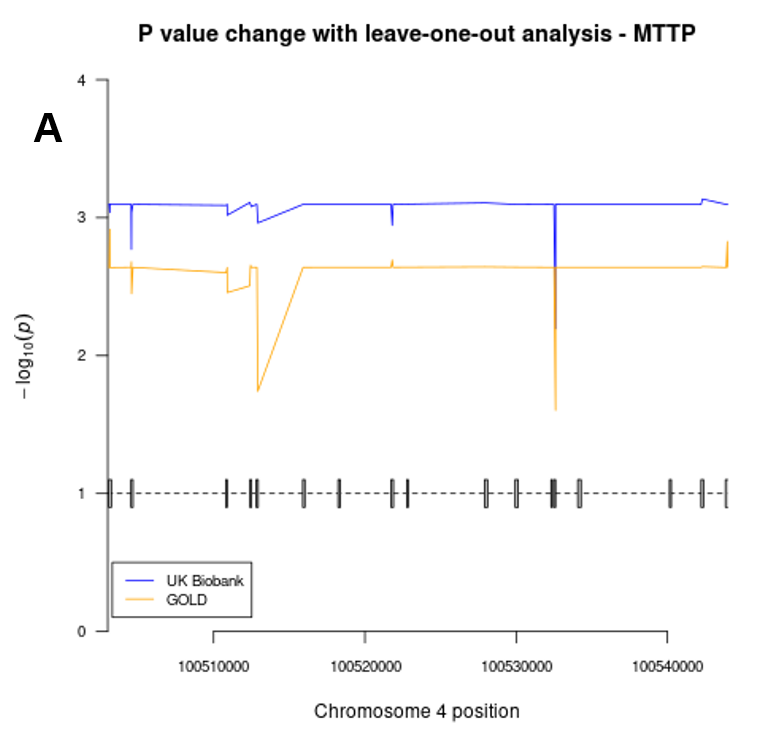
\includegraphics[width=1.0\linewidth]{"images/fig2.png"} 
  \caption{\textbf{Leave One Variant Out plot} (from Du et al 2021). Vertical drops signify associated single variants. V's signify regions of associating rare variants}
  \label{fig:f2}
\end{wrapfigure}
  
We can then apply any peak-finding algorithm (like golden search or derivative approaches) to identify which variants and where along the gene resulted in large peaks of association signal change. This will help identify if the effects of the protein-altering variants are restricted to a specific region of the gene or not. We can then isolate specific regions of a gene and potential polypeptide sequences to study for follow-up analysis.

To verify that we have identified specific causal locations within a gene we can construct a gene-based test using only our implicated causal locations and identifying if the association improves or gets worse. If we do identify a singular causal region we expect the gene-based association p-value to improve (become more significant). If the causal region of the gene cannot be well defined then we expect the gene-based association to perform worse. Based on the positions of the left-most and right-most variants we can produce an estimate of the endpoints for the important MetS loci within an associated gene.

If the loci lies in the exons of a gene and results in a missense or loss-of-function mutation, we can even simulate the folded mutated protein using AlphaFold2 to assess hydrophobic and hydrophilic region changes across the proteins helping inform future functional studies for potential assays and tests to run with these results.

We expect to have a list of genomic endpoints for each gene implicating the deleterious or important parts of a gene relating to MetS. 

\noindent \underbar{Potential Pitfalls \& Alternative Approaches:}

It is possible that after performing the LOVO studies on the genes that no loci across the genes appears to be enriched for MetS association. The LOVO studies produce flat bars or just a lone single peak. In that case, we cannot identify a single causal region. In that case we can include the multiple implicated endpoints for each peak or block. Otherwise we can just encapsulate the entire gene as entirely critical for rare variant association.

Another limitation to this approach is that it assumes that signals associated with variants at a particular locus are due to that region and that region alone. It could be possible that cis or trans effects from other entities associate with the implicated loci, and those might not be detectable through exon sequencing. Functional validation in vitro would be required to followup on the implicated MetS within gene loci; however, we can verify that the implicated loci do not associate with other genetic data like DNA methylation markers instead or additional causes of misclassification.

\subsection*{Aim 2b: Design CRISPR CAS9 KO guides based on exonic variants.} 

\noindent \underbar{Rationale:}

Following 2a we have identified specific regions of interest with our MetS implicated genes. Current functional tests run cellular assays while attempting to remove large coding sections of genes to induce a complete gene knockout in which case the cell can no longer produce that gene on its own. However the concern of regions of a gene affecting the phenotype through mutation of the protein and not simply its absence are still valid. For example consider the case of the Id family of proteins which can affect a phenotype by forming heterodimers with proteins that were expected to homodimerize. Current CRISPR-associated Protien9 (CAS9) knockout tools such as CRISPOR or CHOPCHOP seek to use multiple single-guide RNA (sgRNA) all throughout the gene via a process known as multi-guide mutagenesis. This effectively chops up the gene at various different locations ideally resulting complete gene knockouts. From 2a we have identified specific susceptible MetS regions within a gene. We hypothesize that using a subset of sgRNA CAS9 guides focusing on loci of interest to instead of removing the entire gene, just remove the associated loci of the gene could prove useful for functional validation of these MetS genes and aid in future studies.

\noindent \underbar{Approach:}

There are a plethora of tools for single-guide RNA (sgRNA) design for gene knockout experiments such as CRISPOR or CHOPCHOP, and we can start by using them to generate a list of potential gene knockout guides for each implicated gene. This will form the initial library for MetS functional KO guides.

Then for the genes from 2a of whom we were able to identify specific within gene sequences, we can further filter and assess the recommended guides to help build a more focused MetS gene knockout library. We can use base positioning of the guides to make sure that they only delete the implicated loci for that gene. We can then verify using a tool like CRISPick to obtain an estimate for how efficacious these sets of guides would be at assuring on target knockouts for the selected gene. 

For loci with low probabilities of on target knockout defined as having $<$ 80\% chance for on target efficiency we can default to the originally produced lists of guides and label those sets of guides as full gene knockouts instead of loci specific knockouts. The benefit of this library compared to a standard gene knockout library is the added ability to conduct partial knockouts to study not only the effect of gene omission but a targeted region-specific mutation of a MetS-implicated gene.

At the end, we expect to receive a set of sequences for each MetS-implicated gene that can directly be applied to a functional study of MetS for an in-vitro model.

\noindent \underbar{Potential Pitfalls \& Alternative Approaches:}

This approach has plenty of limitations and makes fundamental assumptions about the CAS9 gene editing process which may not hold true in practice. This approach assumes that CAS9 cutting is precise, but experimentally the guides can perform cuts multiple base pairs away from the intended location which can lead to frameshift mutations resulting in behavior similar to a full gene knockout instead of a focused locus based knockout. Using a tool like CRISPick can help identify rapidly if a specific target set of guides will likely not be effective at producing the intended knockouts, but further in vitro validations should be conducted to ensure that the constructed MetS loci specific CAS9 guide library is effective.

Furthermore, it may be possible that for a given locus no guides can be automatically constructed due to high amounts of genomic repeats or non-uniquely identifiable guide sequences. Usually these tools limit the sgRNA guides to 20 base-pairs; however, an alternative would be to generate longer potential guide sequences of up to 40 base-pairs instead. The longer guide sequences will be more costly to assemble but can help ensure sequence specificity.

\subsection*{Potential Outcomes and Conclusions}

Across these aims we plan to use WES data from the UKBB and MGI to conduct rare-variant association tests to identify novel MetS implicating genes and provide a template for future functional studies. From aim 1a we will obtain a list of novel genes significant for each of the 5 characteristics of MetS based on results from rare variant associations. From aim 1b we will obtain a further refined list of genes whose rare variants are associated with MetS directly along with a more holistic understanding of how individual factors contribute to MetS disease and risk of adverse MetS related outcomes. From aim 2b we expect to have a list of genomic endpoints for each gene implicating the deleterious or important parts of a gene relating to MetS. Finally, from aim 2b we expect to receive a set of sequences for each MetS-implicated gene that can directly be applied to a functional study of MetS for an in-vitro model or assay for MetS.

Major limitations of this approach is that although the variants to be implicated are guaranteed to be exonic and lie within genes, these variants may not cause the phenotypic effects observed. They might tend to associate with other unobserved confounders for MetS. But regardless this approach will help understand the role that rare variants play on MetS while setting up future studies to better understand the biologly behind genetic associations of MetS.

\newpage

\bibliography{proposal} 
\bibliographystyle{ieeetr}

\end{document}